\documentclass[../main.tex]{subfiles}


\begin{document}
\raggedright

\subsection{Basic Web}

	\begin{figure}[H]
        \center{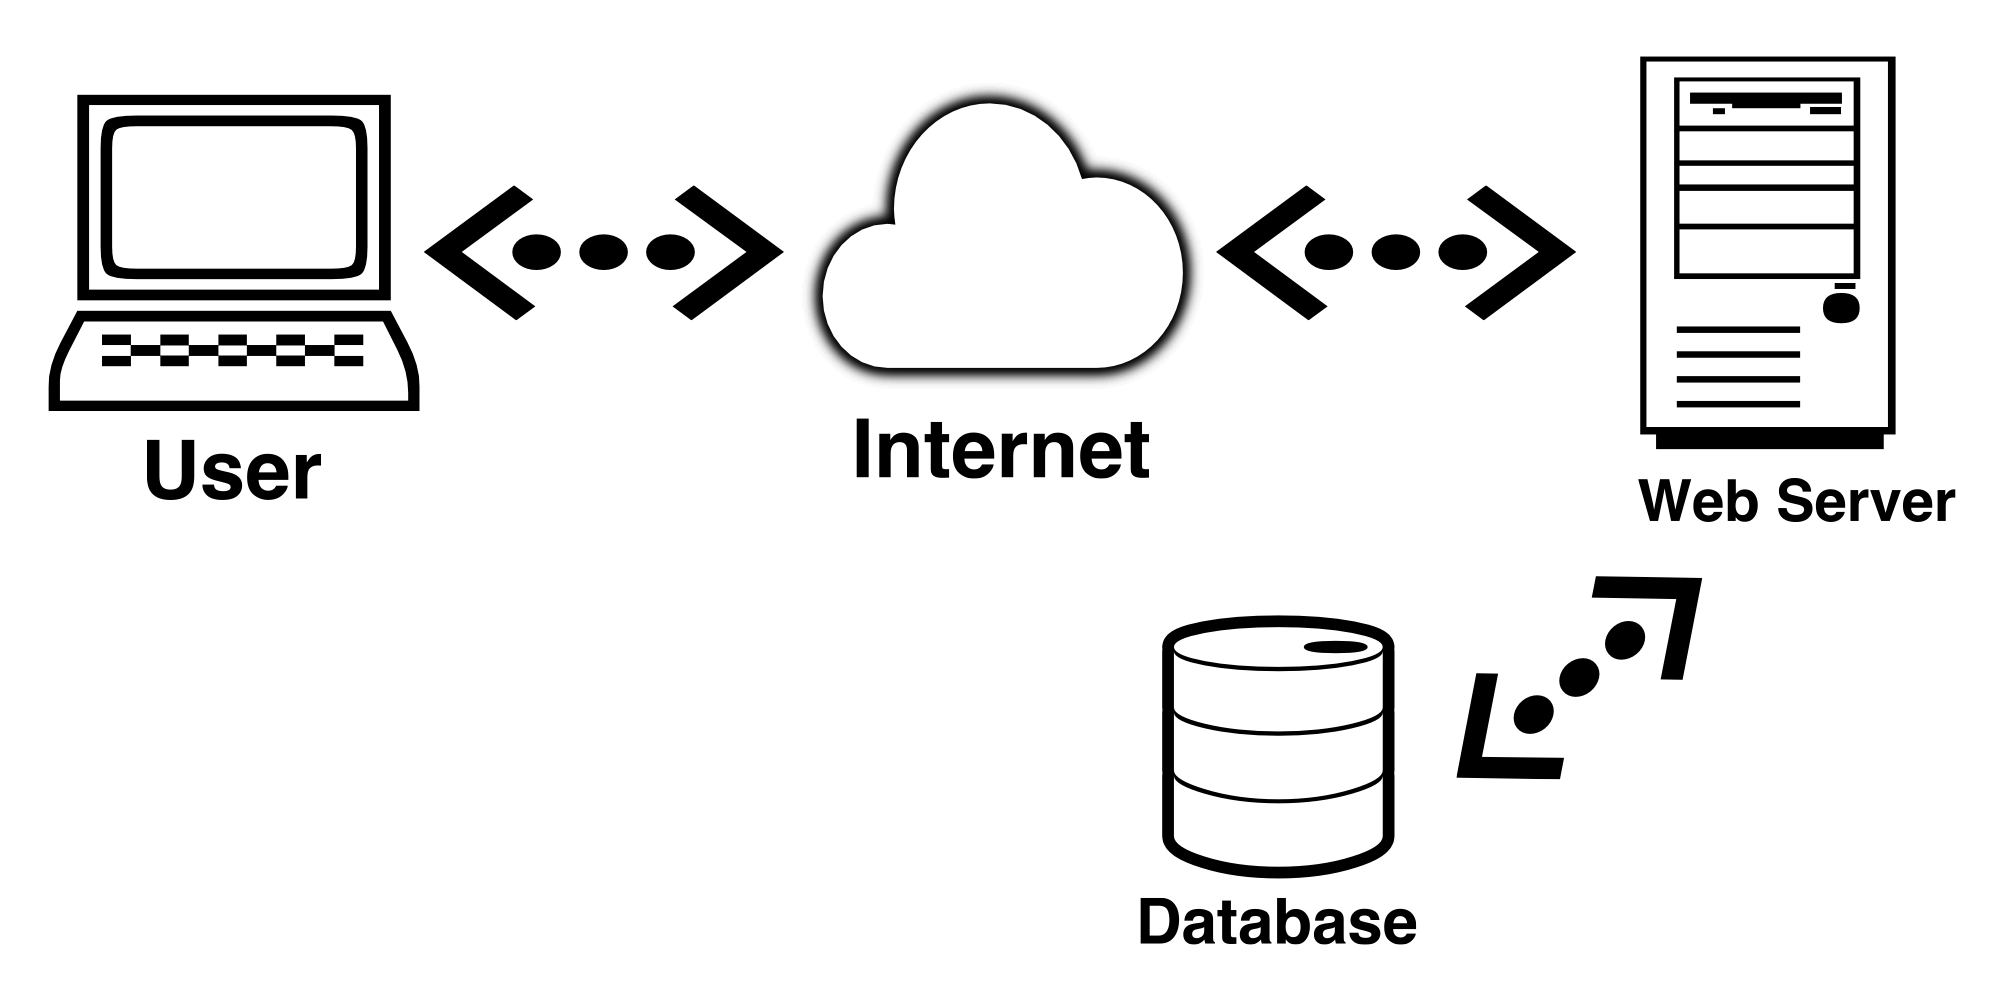
\includegraphics[scale=0.25]
        {images/webserverdesign.png}}
        \caption{\label{fig:basicwebdesign} Basic Web Server.}
      \end{figure}
      
Figure~\ref{fig:basicwebdesign} shows the basic version of how a web server works. The user makes a \textit{request} via their Internet Service Provider(ISP) onto the internet, and that then connects to the web server hosting the site built and the database connected to it. Once the relevant information has been retrieved the server forwards it back to the internet, and the user receives it. Having a system like this would allow the user to access all data from any device, screen size, and hardware that can connect to the internet making it very flexible and easy to use. Security would need to be an essential aspect. 
      
\subsection{The System}
      
Web-Based systems use different languages with both positives and negatives. Java, .NET, PHP, ASP, Python, Ruby, ColdFusion, are just a few of the most used language examples for web systems\cite{securelanguage}. Figure~\ref{fig:mostlanguagesused} and Figure~\ref{fig:languageattacks} shows us programming languages widely used for web systems and a comparison of their vulnerabilities. Selecting a secure language is an important aspect for security and confidentiality of this project.  \\[2mm]


\begin{figure}[H]
        \center{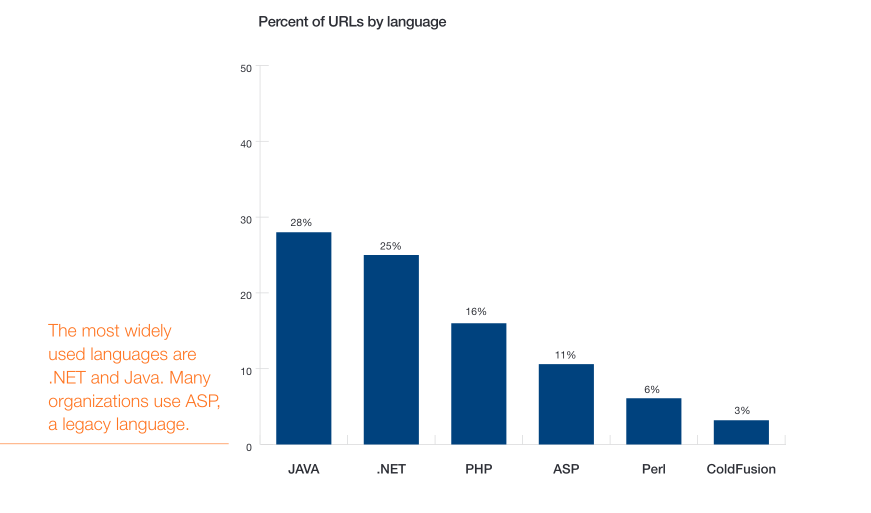
\includegraphics[scale=0.8]
        {images/mostLanguagesUsed.png}}
        \caption{\label{fig:mostlanguagesused} Most widely used languages for Web Systems - WhiteHatSec\cite{WhiteHatSec}}
      \end{figure}


\begin{figure}[H]
        \center{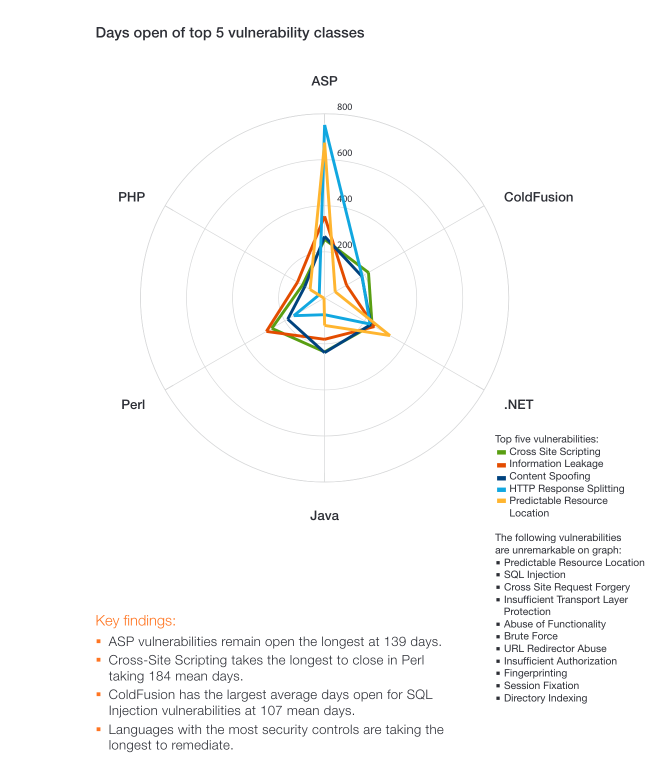
\includegraphics[scale=0.95]
        {images/languageAttacks.png}}
        \caption{\label{fig:languageattacks} Security Vulnerabilites in ASP, PHP, Perl, Java, .NET and ColdFusion - WhiteHatSec\cite{WhiteHatSec}}
      \end{figure}
      
With all these languages, the highest priority would be to find a language which has cybersecurity as one of its main components. A huge number of programmers use .NET, Java, ASP, PHP and hence they come with a high number of vulnerabilities making them highly maintainable and certainly less secure.\cite{securelanguage}. Python which is another highly used programming language is said to have more security than some of its alternates; this is due to the huge community and preference of cyber researchers.\cite{topfivecyber}  \\[4mm]

All the above are regular languages which have a framework under web development. Python has Django; Ruby has Ruby on Rails, JavaScript has NodeJS and many others. Each of these can help develop a system with similar functions, but not all can provide the same levels of security, speed or scalability.\cite{djangovslaravel}\cite{webdev}. 




\end{document}
